\documentclass{article}

  % packages
    % basic stuff for rendering math
    \usepackage[letterpaper, top=1in, bottom=1in, left=1in, right=1in]{geometry}
    \usepackage[utf8]{inputenc}
    \usepackage[english]{babel}
    \usepackage{amsmath} 
    \usepackage{amssymb}
    % \usepackage{amsthm}

    % extra math symbols and utilities
    \usepackage{mathtools}        % for extra stuff like \coloneqq
    \usepackage{mathrsfs}         % for extra stuff like \mathsrc{}
    \usepackage{centernot}        % for the centernot arrow 
    \usepackage{bm}               % for better boldsymbol/mathbf 
    \usepackage{enumitem}         % better control over enumerate, itemize
    \usepackage{hyperref}         % for hypertext linking
    \usepackage{fancyvrb}          % for better verbatim environments
    \usepackage{newverbs}         % for texttt{}
    \usepackage{xcolor}           % for colored text 
    \usepackage{listings}         % to include code
    \usepackage{lstautogobble}    % helper package for code
    \usepackage{parcolumns}       % for side by side columns for two column code
    

    % page layout
    \usepackage{fancyhdr}         % for headers and footers 
    \usepackage{lastpage}         % to include last page number in footer 
    \usepackage{parskip}          % for no indentation and space between paragraphs    
    \usepackage[T1]{fontenc}      % to include \textbackslash
    \usepackage{footnote}
    \usepackage{etoolbox}

    % for custom environments
    \usepackage{tcolorbox}        % for better colored boxes in custom environments
    \tcbuselibrary{breakable}     % to allow tcolorboxes to break across pages

    % figures
    \usepackage{pgfplots}
    \pgfplotsset{compat=1.18}
    \usepackage{float}            % for [H] figure placement
    \usepackage{tikz}
    \usepackage{tikz-cd}
    \usepackage{circuitikz}
    \usetikzlibrary{arrows}
    \usetikzlibrary{positioning}
    \usetikzlibrary{calc}
    \usepackage{graphicx}
    \usepackage{algorithmic}
    \usepackage{caption} 
    \usepackage{subcaption}
    \captionsetup{font=small}

    % for tabular stuff 
    \usepackage{dcolumn}

    \usepackage[nottoc]{tocbibind}
    \pdfsuppresswarningpagegroup=1
    \hfuzz=5.002pt                % ignore overfull hbox badness warnings below this limit

  % New and replaced operators
    \DeclareMathOperator*{\card}{card}
    \DeclareMathOperator*{\argmin}{\arg\!\min}
    \DeclareMathOperator*{\argmax}{\arg\!\max}
    \newcommand{\qed}{\hfill$\blacksquare$}     % I like QED squares to be black

  % Custom Environments
    \newtcolorbox[auto counter, number within=section]{question}[1][]
    {
      colframe = orange!25,
      colback  = orange!10,
      coltitle = orange!20!black,  
      breakable, 
      title = \textbf{Question \thetcbcounter ~(#1)}
    }

    \newtcolorbox[auto counter, number within=section]{exercise}[1][]
    {
      colframe = teal!25,
      colback  = teal!10,
      coltitle = teal!20!black,  
      breakable, 
      title = \textbf{Exercise \thetcbcounter ~(#1)}
    }
    \newtcolorbox[auto counter, number within=section]{solution}[1][]
    {
      colframe = violet!25,
      colback  = violet!10,
      coltitle = violet!20!black,  
      breakable, 
      title = \textbf{Solution \thetcbcounter}
    }
    \newtcolorbox[auto counter, number within=section]{lemma}[1][]
    {
      colframe = red!25,
      colback  = red!10,
      coltitle = red!20!black,  
      breakable, 
      title = \textbf{Lemma \thetcbcounter ~(#1)}
    }
    \newtcolorbox[auto counter, number within=section]{theorem}[1][]
    {
      colframe = red!25,
      colback  = red!10,
      coltitle = red!20!black,  
      breakable, 
      title = \textbf{Theorem \thetcbcounter ~(#1)}
    } 
    \newtcolorbox[auto counter, number within=section]{proposition}[1][]
    {
      colframe = red!25,
      colback  = red!10,
      coltitle = red!20!black,  
      breakable, 
      title = \textbf{Proposition \thetcbcounter ~(#1)}
    } 
    \newtcolorbox[auto counter, number within=section]{corollary}[1][]
    {
      colframe = red!25,
      colback  = red!10,
      coltitle = red!20!black,  
      breakable, 
      title = \textbf{Corollary \thetcbcounter ~(#1)}
    } 
    \newtcolorbox[auto counter, number within=section]{proof}[1][]
    {
      colframe = orange!25,
      colback  = orange!10,
      coltitle = orange!20!black,  
      breakable, 
      title = \textbf{Proof. }
    } 
    \newtcolorbox[auto counter, number within=section]{definition}[1][]
    {
      colframe = yellow!25,
      colback  = yellow!10,
      coltitle = yellow!20!black,  
      breakable, 
      title = \textbf{Definition \thetcbcounter ~(#1)}
    } 
    \newtcolorbox[auto counter, number within=section]{example}[1][]
    {
      colframe = blue!25,
      colback  = blue!10,
      coltitle = blue!20!black,  
      breakable, 
      title = \textbf{Example \thetcbcounter ~(#1)}
    } 
    \newtcolorbox[auto counter, number within=section]{axiom}[1][]
    {
      colframe = green!25,
      colback  = green!10,
      coltitle = green!20!black,  
      breakable, 
      title = \textbf{Axiom \thetcbcounter ~(#1)}
    } 
    \newtcolorbox[auto counter, number within=section]{algo}[1][]
    {
      colframe = green!25,
      colback  = green!10,
      coltitle = green!20!black,  
      breakable, 
      title = \textbf{Algorithm \thetcbcounter ~(#1)}
    } 

    \BeforeBeginEnvironment{example}{\savenotes}
    \AfterEndEnvironment{example}{\spewnotes}
    \BeforeBeginEnvironment{lemma}{\savenotes}
    \AfterEndEnvironment{lemma}{\spewnotes}
    \BeforeBeginEnvironment{theorem}{\savenotes}
    \AfterEndEnvironment{theorem}{\spewnotes}
    \BeforeBeginEnvironment{corollary}{\savenotes}
    \AfterEndEnvironment{corollary}{\spewnotes}
    \BeforeBeginEnvironment{proposition}{\savenotes}
    \AfterEndEnvironment{proposition}{\spewnotes}
    \BeforeBeginEnvironment{definition}{\savenotes}
    \AfterEndEnvironment{definition}{\spewnotes}
    \BeforeBeginEnvironment{exercise}{\savenotes}
    \AfterEndEnvironment{exercise}{\spewnotes}
    \BeforeBeginEnvironment{proof}{\savenotes}
    \AfterEndEnvironment{proof}{\spewnotes}
    \BeforeBeginEnvironment{solution}{\savenotes}
    \AfterEndEnvironment{solution}{\spewnotes}
    \BeforeBeginEnvironment{question}{\savenotes}
    \AfterEndEnvironment{question}{\spewnotes}
    \BeforeBeginEnvironment{axiom}{\savenotes}
    \AfterEndEnvironment{axiom}{\spewnotes}
    \BeforeBeginEnvironment{algo}{\savenotes}
    \AfterEndEnvironment{algo}{\spewnotes}

    \definecolor{dkgreen}{rgb}{0,0.6,0}
    \definecolor{gray}{rgb}{0.5,0.5,0.5}
    \definecolor{mauve}{rgb}{0.58,0,0.82}
    \definecolor{darkblue}{rgb}{0,0,139}
    \definecolor{lightgray}{gray}{0.93}
    \renewcommand{\algorithmiccomment}[1]{\hfill$\triangleright$\textcolor{blue}{#1}}

    % default options for listings (for code)
    \lstset{
      autogobble,
      frame=ltbr,
      language=Python,
      aboveskip=3mm,
      belowskip=3mm,
      showstringspaces=false,
      columns=fullflexible,
      keepspaces=true,
      basicstyle={\small\ttfamily},
      numbers=left,
      firstnumber=1,                        % start line number at 1
      numberstyle=\tiny\color{gray},
      keywordstyle=\color{blue},
      commentstyle=\color{dkgreen},
      stringstyle=\color{mauve},
      backgroundcolor=\color{lightgray}, 
      breaklines=true,                      % break lines
      breakatwhitespace=true,
      tabsize=3, 
      xleftmargin=2em, 
      framexleftmargin=1.5em, 
      stepnumber=1
    }

  % Page style
    \pagestyle{fancy}
    \fancyhead[L]{Set Theory}
    \fancyhead[C]{Muchang Bahng}
    \fancyhead[R]{Spring 2025} 
    \fancyfoot[C]{\thepage / \pageref{LastPage}}
    \renewcommand{\footrulewidth}{0.4pt}          % the footer line should be 0.4pt wide
    \renewcommand{\thispagestyle}[1]{}  % needed to include headers in title page

\begin{document}

\title{Set Theory}
\author{Muchang Bahng}
\date{Spring 2025}

\maketitle
\tableofcontents
\pagebreak

\section{Naive Set Theory}

  Unlike axiomatic set theories, which are defined using formal logic, naive set theory was defined informally at the end of the 19th century by Cantor, in natural language (like English). It describes the aspects of mathematical sets using words (e.g. \textit{satisfying, such as, ...}) and suffices for the everyday use of set theory in modern mathematics. However, as we will see, this leads to paradoxes. 

  \begin{definition}[Set]
    A \textbf{set} is a well-defined collection of distinct objects, called \textbf{elements}. 
  \end{definition}

  This definition tells us \textit{what} a set is, but does not define \textit{how} sets can be formed, and what operations on sets will again produce a set. The term \textit{well-defined} cannot by itself guarantee the consistency and unambiguity of what exactly constitutes and what does not constitute a set, and therefore this is not a formal definition. Attempting to achieve this will be done in axiomatic set theory, like ZFC. 

  \begin{definition}[Membership]
    If $x$ is a member of $A$, we write $x \in A$. For any $x$, it must be the case that either $x \in A$ (exclusive or) $x \not\in A$. 
  \end{definition}
  
  \begin{definition}[Equality]
    Two sets $A$ and $B$ are defined to be equal, denoted as $A = B$, when they have precisely the same elements. That is, if $x \in A \iff x \in B$. This means that a set is completely determined by its elements, and the description is immaterial. 
  \end{definition}

  \begin{definition}[Empty Set]
    There exists an empty set, denoted $\emptyset$ or $\{\}$, which is a set with no members at all. Because a set is described by its elements, there can only be one empty set. 
  \end{definition}

  Now we show how to construct sets. 

  \begin{definition}[Set-Builder Notation]
    We can construct a set in two ways. 
    \begin{enumerate}
      \item We list its elements between curly braces. 
      \begin{enumerate}
        \item The set $\{1, 2\}$ denotes the set containing $1$ and $2$. By equality $\{1, 2\} = \{2, 1\}$. 
        \item Repetition/multiplicity is irrelevant, and so $\{1, 2, 2\} = \{1, 1, 1, 2\} = \{1, 2\}$ 
      \end{enumerate} 

      \item We denote 
      \begin{equation}
        S = \{ x | P(x) \}
      \end{equation} 
      where $P$ is a property. If $x$ satisfies this property, then $x \in S$. 
    \end{enumerate}
    Naive set theory claims that this construction \textit{always} produces a set. Therefore, a well-defined property is enough to always produce a set of elements satisfying $P$. 
  \end{definition} 

  \begin{example}[Empty Set]
    Let $S = \{x \mid x \neq x \}$. For any $x$, $P(x)$ is false and so $S$ contains no elements. Therefore $S = \emptyset$. 
  \end{example}

  \begin{example}[Singleton Set]
    The set $\{x \mid x = a \} = \{a\}$. 
  \end{example}

  \begin{example}[Russell Set]
    Let $R = \{x \mid x \not\in x\}$, i.e. the set of all sets that do not contain themselves as elements. 
  \end{example}

  \begin{theorem}[Russell's Paradox] 
    The Russell set exists and does not exist. 
  \end{theorem}
  \begin{proof}
    We will determine if $R$ is an element of itself. 
    \begin{enumerate}
      \item If $R \in R$, then by it does contain itself, so it does not satisfy the property and $R \not\in R$. 
      \item If $R \not\in R$, then it satisfies the property, so $R \in R$. 
    \end{enumerate}
    Therefore, it is both the case that $x \in R$ and $x \not\in R$, which contradicts the membership definition. Therefore, $R$ is both a set from set-builder construction and not a set due to the membership definition. 
  \end{proof}

  \begin{theorem}[Existence of Universe]
    Let $U$ be the set of everything, known as the \textbf{universal set}. The universal set does exist and does not exist. 
  \end{theorem}
  \begin{proof}
    We can define $U^\prime = \{x \mid \{\} = \{\} \}$, which defines a set. Then the property $P$ that $\{\} = \{\}$ is always true, and $U^\prime$ would contain everything, and by the definition of equality $U = U^\prime$. Now since the Russell set $R$ is both a set and not a set from Russell's paradox, we have $R \in U$ and $R \not\in U$, which means that $U$ cannot exist. Therefore $U$ does not exist. 
  \end{proof}

  So the sufficiency a well-defined property to be able to construct a set is \textit{too powerful} in that we can construct \textit{any} set we want. This leads us to construct the Russell set, which opens up a lot of paradoxes. Therefore, we would like to restrict the notion of well-defined in a way, which leads to axiomatic set theories. 

  \begin{definition}[Subsets]
    Given two sets $A$ and $B$, $A$ is a \textbf{subset} of $B$ if every element of $A$ is also an element of $B$. A subset of $B$ that is not equal to $B$ is called a \textbf{proper subset}. 
  \end{definition}

  \begin{theorem}[Equality]
    It follows from the definition of equality that 
    \begin{equation}
      A \subset B \text{ and } B \subset A \iff A = B
    \end{equation}
  \end{theorem}

  \begin{definition}[Power Set]
    The set of all subsets of a set $A$ is called the \textbf{power set} of $A$, denoted by $2^A$. 
  \end{definition}

  We could define other things like the union, etc., but I won't bother with it when I will define them for ZFC later.  

\section{Zermelo-Fraenkel-Choice (ZFC) Set Theory} 

    So with these paradoxes in mind, we would like to construct an axiomatic formulation of sets. My take is to think that sets ``exist'' out there somewhere in the universe, and our job is to find them. Cantor with his naive set theory believed that for every meaningful property of things there is a set whose members are exactly all the things with that property. Russell shows this this cannot be the case. Nevertheless, \textit{some} sets exist, and we have intuitive experience thinking about finite sets. Therefore, the axioms of set theory are a limited list of \textit{assumptions} that we hope are true about that actually existing universe of sets. As long as they are true, then whatever we conclude from them by valid reasoning steps must also be true.\footnote{This idea is called naive Platonism.} Hence we have the following definition, which first requires the familiar property of acting like a collection of something, and then obeys the axioms we set. 
    
    \begin{definition}[Set]
      A \textbf{set} $X$ is anything 
      \begin{enumerate}
        \item that has the innate property of containing elements, and 
        \item obeys the axioms of ZFC. 
      \end{enumerate}
    \end{definition}  

    Let's first talk about the language, where they are defined formally using the axioms in the next subsection. From first-order logic, note that we have the following symbols in our alphabet $\mathcal{L}_{\mathrm{ZFC}}$. 
    \begin{enumerate}
      \item The logical connectives $\neg$, $\lor$, $\land$. 
      \item The quantifier symbols $\exists, \forall$ 
      \item Brackets $()$. 
    \end{enumerate}
    To represent sets, we also need symbols, and the membership property requires us to define a symbol for that too. 
    \begin{enumerate}
      \item A countably infinite amount of variables used for representing sets. 
      \item The set membership symbol $\in$. In fact, when we say $x \in A$, this is a proposition formed from the predicate $P(x)$. 
    \end{enumerate} 
    This is what we have to work with so far. We will construct the rest of the symbols ($=, \subset, \supset, \cup, \cap$) from the axioms. So far we don't even know if there exists any set that obeys the following axioms! Therefore, we will assert the existence of at least one set, namely the empty set. 

  \subsection{ZF Axioms}

    Now we state the axioms, which is the foundation of ZF set theory. 

    \begin{axiom}[Empty Set]
      The empty set containing no elements exists. 
    \end{axiom}

    \begin{definition}[Empty Set]
      The empty set is denoted $\emptyset$. 
    \end{definition}

    This asserts the existence of at least 1 set, which we will build on to create more sets. 

    \begin{axiom}[Axiom of Extensionality]
      Two sets are equal (are the same set) if they have the same elements. 
      \begin{equation}
        \forall A \forall B \big[ \forall x (x \in A \iff x \in B) \iff A = B\big]
      \end{equation}
    \end{axiom} 

    \begin{definition}[Equality]
      This axiom allows us to define the equality operator $=$, which we now add to our alphabet. 
    \end{definition}

    \begin{theorem}[Sets Don't Contain Repeated Elements]
      Furthermore, this axiom also implies that sets are unique up to distinct elements. That is, 
      \begin{equation}
        \{1, 1, 2\} = \{1, 2\} = \{1, 1, 2, 2\}
      \end{equation}
    \end{theorem}

    \begin{axiom}[Axiom of Regularity]
      Every non-empty set $A$ contains a member $x$ such that $A$ and $x$ are disjoint sets. 
      \begin{equation}
        \forall A \big[ A \neq \emptyset \implies \exists x (x \in A \land A \cap x = \emptyset) \big]
      \end{equation}
      This, along with the axioms of pairing and union, implies that no set is an element of itself and that every set has an ordinal rank. 
    \end{axiom}

    The axiom assists us in regulating which sets are viable and which are not, preventing Russell's paradox. 

    \begin{axiom}[Axiom Schema of Restricted Comprehension, or Specification]
      Subsets, like in naive set theory, are constructed using set builder notation. In general, the \textbf{subset} of a set $A$ obeying a formula $\phi(x)$ with one free variable $x$ may be written as 
      \begin{equation}
        \{x \in A \mid \phi(x) \}
      \end{equation}
      The axiom schema of specification states that this subset always exists.\footnote{Note that this axiom does not allow the construction of entities of the more general form $\{x \mid \phi(x)\}$. This restriction is obviously needed to avoid Russell's paradox, hence the name \textit{restricted} comprehension. } 
    \end{axiom}  

    \begin{definition}[Subset, Superset]
      The axiom of specification allows us to denote subsets. Notationally, if $A$ is a subset of $B$, then we write $A \subset B$. Similarly, we say $A$ is a \textbf{superset} of $B$, written $A \supset B$, if $B \subset A$. 
    \end{definition} 
    
    \begin{definition}[Intersection]
      This also allows us to define intersection as 
      \begin{equation}
        A \cap B \coloneqq \{x \in A \mid x \in B \}
      \end{equation} 
      and we can define the intersection of an arbitrary collection of sets $\mathcal{F}$ as the following. Let $A \in \mathcal{F}$.  
      \begin{equation}
        \bigcap \mathcal{F} \coloneqq \{x \in A \mid \forall B (B \in \mathcal{F} \implies x \in B) \}
      \end{equation}
    \end{definition}

    Unfortunately, the union cannot be expressed in this specification schema, and we need a separate axiom for this. 

    \begin{definition}[Set Minus]
      We can however define set minus. Given sets $A, B$
      \begin{equation}
        A \setminus B \coloneqq \{ x \in A \mid x \not\in B \}
      \end{equation}
    \end{definition}

    \begin{definition}[Set Complement]
      Given $B$ and a subset $A \subset B$, the \textbf{complement} of $A$ with respect to $B$ is 
      \begin{equation}
        A^c \coloneqq \{ x \in B \mid x \not\in A \} = B \setminus A
      \end{equation}
    \end{definition}

    \begin{axiom}[Axiom of Pairing]
      If $A, B$ are sets, then there exists a set which contains $A$ and $B$ as elements.\footnote{For example, if $A = \{1, 2\}$ and $B = \{2, 3\}$,then $\{\{1, 2\}, \{2, 3\}\}$ exists.}
      \begin{equation}
        \forall A \forall B \exists C((A \in C) \land (B \in C))
      \end{equation}
      This allows us to construct sets from old ones. 
    \end{axiom}

    \begin{theorem}[Nested Sets]
      By the axiom of pairing, if we have a set $X$, then $\{X\}$ is also a set, since we can set $A = B = X$ which asserts the existence of $\{X, X\} = \{X\}$. 
    \end{theorem}

    \begin{axiom}[Axiom of Union]
      For any set of sets $\mathcal{F}$, there is a set $A$ containing every element that is a member of $\mathcal{F}$.
      \begin{equation}
        \forall \mathcal{F} \exists A \forall X \forall x \big[ (x \in X \land X \in \mathcal{F}) \implies x \in A \big]
      \end{equation}
    \end{axiom}

    This formula doesn't directly assert the existence of $\cup \mathcal{F}$ (?). 

    \begin{definition}[Union]
      The set $\cup \mathcal{F}$ can be constructed from $A$ in the above using the axiom schema of restricted comprehension. 
      \begin{equation}
        \cup \mathcal{F} = \{ x \in A \mid \exists X (x \in X \land X \in \mathcal{F} ) \}
      \end{equation}
    \end{definition}

    \begin{axiom}[Axiom of Infinity]
      The axiom of infinity guarantees the existence of at least one infinite set. That is, given a set $w$, let $S(w) = w \cup \{w\}$ be a set.\footnote{Since $w$ is a set, by the axiom of pairing $\{w\}$ is a set, and by the axiom of union $w \cup \{w\}$ is a set.} Then, there exists a set $X$ such that 
      \begin{enumerate}
        \item $\emptyset \in X$, and 
        \item if $w \in X$, then $S(w) \in X$. 
      \end{enumerate} 
      In logic terms, 
      \begin{equation}
        \exists X \big[ \emptyset \in X \land \forall y (y \in X \implies S(y) \in X) \big]
      \end{equation}
      Since we have axiomatically claimed the two premises to be true, by propositional logic, namely \textit{modus ponens}, this implies the existence of at least one set $X$ with infinitely many members. 
    \end{axiom}

    \begin{definition}[Von Neumann Ordinals] 
       The \textbf{Von Neumann ordinals} is the minimal set $X$ satisfying the axiom of infinity. It is the set containing 
      \begin{align*}
        0 & = \{\} = \emptyset \\
        1 & = \{0\} = \{\emptyset\} \\
        2 & = \{0,1\} = \{\emptyset,\{\emptyset\}\} \\
        3 & = \{0,1,2\} = \{\emptyset,\{\emptyset\},\{\emptyset,\{\emptyset\}\}\} \\
        4 & = \{0,1,2,3\} = \{\emptyset,\{\emptyset\},\{\emptyset,\{\emptyset\}\},\{\emptyset,\{\emptyset\},\{\emptyset,\{\emptyset\}\}\}\} \\
        \ldots & = \ldots 
      \end{align*} 
      This provides the foundation to construct the most basic mathematical sets: the natural numbers denoted $\mathbb{N}$.  
    \end{definition} 

    Now that we have constructed the Von Neumann ordinals, we are allowed to do \textit{indexing}. 

    \begin{axiom}[Axiom of Power Set]
      The axiom of power set states that for any set $A$, there is a set $B$ that contains every subset\footnote{Note that subset is defined by the axiom of restricted comprehension.} of $A$. 
      \begin{equation}
        \forall A \exists B \forall S (S \subset A \implies S \in B)
      \end{equation}
      The axiom of schema of specification is then used to define the power set as the subset of such $B$ containing the subset of $A$ exactly. 
      \begin{equation}
        2^X = \{Y \in B \mid Y \subset X \}
      \end{equation}
    \end{axiom} 

    \begin{definition}[Cartesian Product]
      The power set axiom allows for the definition of the \textbf{Cartesian product} of two sets $X$ and $Y$. Note that if $x \in X, y \in Y$, then by the axiom of union $x, y \in X \cup Y$ and by the axiom of power set $\{x\}, \{x, y\} \in \mathcal{P}(X \cup Y)$. Therefore, using the axiom of power set again we can define
      \begin{equation}
        (x, y) \coloneqq \{\{x\}, \{x, y\}\} \in \mathcal{P}(\mathcal{P}(X \cup Y))
      \end{equation} 
      and the Cartesian product is defined 
      \begin{equation}
        X \times Y \coloneqq = \{ (x, y) \in \mathcal{P}(\mathcal{P}(X \cup Y))  \mid x \in X \land y \in Y \}
      \end{equation}
      which is axiomatically a valid set by the axiom schema of specification. 
    \end{definition} 

    From this we can define the Cartesian product of any finite collection of sets recursively. It is indeed the case that $(X \times Y) \times Z$ is a different set from $X \times (Y \times Z)$, but as we will see in later functions, we can define a canonical bijection between them, treating them as equivalent. Furthermore, notice that we have not defined the Cartesian product of infinite sets yet. We can define them using functions actually. 

  \subsection{Functions} 

    The definition of Cartesian products allows us to formally define \textbf{correspondences}. The most notable correspondences are \textit{functions} and \textit{relations}. 

    \begin{definition}[Function]
      Given two sets $X, Y$, a function $f: X \rightarrow Y$ is a subset $f \subset X \times Y$ satisfying the following
      \begin{enumerate}
        \item For all $x \in X$, there exists $y \in Y$ s.t. $(x, y) \in f$.\footnote{This says that $f$ must be defined for all inputs in $X$.}
        \item For all $x \in X$ and $y, y^\prime \in Y$, if $(x, y) \in f$ and $(x, y^\prime) \in f$, then $y = y^\prime$.\footnote{In other words, $f$ must map one element to exactly one element.} 
      \end{enumerate}
      The set $X$ is said to be the \textbf{domain} and $Y$ the \textbf{codomain}. 

      \begin{figure}[H]
        \centering 
        \begin{tikzcd}
          X \arrow[r, "f"'] & Y 
        \end{tikzcd}
        \caption{A diagram representing the function $f: X \rightarrow Y$.} 
        \label{fig:function at}
      \end{figure}
    \end{definition}  

    \begin{definition}[Image, Preimage]
      Given some $f: X \rightarrow Y$ and $A \subset X$, the \textbf{image} of $A$ under $f$ is defined 
      \begin{equation}
        f(A) \coloneqq \{y \in Y \mid \exists x \in X (f(x) = y)\}
      \end{equation}
      Given $B \subset Y$, the \textbf{preimage} of $B$ under $f$ is defined 
      \begin{equation}
        f^{-1} (B) \coloneqq \{ x \in X \mid f(x) \in B \}
      \end{equation}
    \end{definition} 

    \begin{axiom}[Axiom Schema of Replacement]
      This axiom asserts that the image of a set under any definable function will fall inside a set. 
    \end{axiom} 

    Again, how do we even know for sure that these axioms aren't contradictory? The answer is that we don't, and that is why we take them as axioms rather than provable theorems. Fortunately, from the formulation in the early 20th century up until now, no contradictions have been found, and if there is one, then it would be very bad news for us.  

    \begin{definition}[Injectivity, Surjectivity, Bijectivity]
      A function $f: X \rightarrow Y$ is said to be 
      \begin{enumerate}
        \item \textbf{injective} if $\forall x \in X, \forall x^\prime \in X \big( f(x) = f(x^\prime) \implies x = x^\prime \big)$. 
        \item \textbf{surjective} if $\forall y \in Y \exists x \in X (y = f(x))$. 
        \item \textbf{bijective} if it is injective and surjective. 
      \end{enumerate}
    \end{definition}

    \begin{definition}[Inverse Function]
      If a function $f: X \rightarrow Y$ is bijective, then there exists an \textbf{inverse function} $f^{-1}: Y \rightarrow X$ satisfying 
      \begin{equation}
        \forall x \in X \big[ f(f^{-1}(x)) = f^{-1} (f(x)) = x \big]
      \end{equation}
    \end{definition} 

    \begin{definition}[Restriction]
      If $f: X \rightarrow Y$ and $X_0 \subset X$, we define the \textbf{restriction} of $f$ to $X_0$ to be the function mapping to $Y$ whose rule is 
      \begin{equation}
        f|_{X_0} \coloneqq \{ (x, f(x)) \in f x \in X_0 \}
      \end{equation}
    \end{definition} 

    \begin{definition}[Composition]
      Given functions $f: X \rightarrow Y$, $g: Y \rightarrow Z$, we define the \textbf{composite}, denoted $g \circ f$ or $g(f(\cdot))$, of $f$ and $g$ as the subset
      \begin{equation}
        g \circ f \coloneqq \{ (x, z) \in X \times Z \mid \exists y \in Y (f(x) = y \land f(y) = z) \}
      \end{equation} 
    \end{definition}

    \begin{theorem}[Compositions]
      A composite is a function. 
      \begin{figure}[H]
        \centering 
        \begin{tikzcd}
          X \arrow[r, "f"] \arrow[rd, "g \circ f"'] & Y \arrow[d, "g"] \\
          & Z
        \end{tikzcd}
        \caption{Commutative diagram representing a composition of functions.} 
        \label{fig:composition}
      \end{figure}
    \end{theorem}
    \begin{proof}
      Using the definition above, we prove the two properties. 
      \begin{enumerate}
        \item For all $x \in X$, there exists $y \in Y$ s.t. $(x, y) \in f$. Similarly, for all $y \in Y$, there exists $z \in Z$ s.t. $(y, z) \in g$. Therefore, for all $x \in X$, there exists a $y \in Y$, which follows that there exists also a $z \in Z$. Therefore $g \circ f$ is defined for all inputs in $X$. 
        \item For all $x \in X$ and $z, z^\prime \in Z$, say that $(x, z), (x, z^\prime) \in g \circ f$. Then by definition of composition there exists a $y, y^\prime \in Y$ s.t. $f(x) = y, f(y) = z$ and $f(x) = y^\prime, f(y^\prime) = z^\prime$. Since $f$ is a function, $y = y^\prime$. Since $g$ is a function, $y = y^\prime \implies z = z^\prime$. Therefore $g \circ f$ is a function. 
      \end{enumerate}
    \end{proof}

    For the computer science students, note that a function behaves precisely like functional dependencies in a relational database. A composition represents a natural join. 

    \begin{theorem}[Associativity]
      Composition is associative. That is, consider $f: Y \rightarrow Z, g: X \rightarrow Y, h: W \rightarrow X$ functions. Then 
      \begin{equation}
        (f \circ g) \circ h = f \circ (g \circ h)
      \end{equation} 
      Therefore, we write this as 
      \begin{equation}
        f \circ g \circ h
      \end{equation} 
      \begin{figure}[H]
        \centering 
        \begin{tikzcd}
          & X \arrow[r, "g"] \arrow[rrd, "g \circ h"'] & Y \arrow[rd, "h"] & \\ 
          W \arrow[ru, "f"] \arrow[rru, "g \circ f"'] & & & Z 
        \end{tikzcd}
        \caption{} 
        \label{fig:associative}
      \end{figure}
    \end{theorem}
    \begin{proof}
      Consider any $w \in W$, and let us label $x = h(w)$, $y = g(x)$, $z = f(y)$, where $x, y, z$ must be uniquely determined by $w$ since it is a function. Then, 
      \begin{align}
        ((f \circ g) \circ h) (w) & = (f \circ g) (h(w)) = (f \circ g) (x) = z  \\
        (f \circ (g \circ h)) (w) & = f ((g \circ h)(w)) = f (y) = z
      \end{align}
      and they coincide for all $w \in W$. 
    \end{proof} 

    If we are familiar with algebra, this gives the set of functions $\{f: X \rightarrow X\}$ the structure of a \textit{monoid} under composition. We can also talk about commutativity. 

    \begin{definition}[Commutativity]
      Two functions $f, g: X \rightarrow X$ are said to be \textbf{commute} if 
      \begin{equation}
        f \circ g = g \circ f
      \end{equation} 
      \begin{figure}[H]
        \centering 
        \begin{tikzcd}
          X \arrow[r, "f"] \arrow[d, "g"] & X \arrow[d, "g"] \\
          X \arrow[r, "f"] & X 
        \end{tikzcd}
        \caption{Commutative diagram representing commuting functions $f, g$. } 
        \label{fig:commutative}
      \end{figure}
    \end{definition}

  \subsection{Relations}

    \begin{definition}[Relation]
      A binary relation $R$ on a set $A$ is a subset of $A \times A$. We write $aRb$ if and only if $(a,b) \in R$.\footnote{It is a way of describing precisely which two elements are related to one another.} 
    \end{definition} 

    But not all relations may be meaningful or interesting. Therefore we usually like to have certain properties on these relations. 
    \begin{enumerate}
      \item \textit{Reflexive}. For all $a \in A$, $aRa$
      \item \textit{Symmetric}. For all $a,b \in A$, if $aRb$ then $bRa$
      \item \textit{Antisymmetric}. For all $a,b \in A$, if $aRb$ and $bRa$ then $a=b$
      \item \textit{Transitive}. For all $a,b,c \in A$, if $aRb$ and $bRc$ then $aRc$
      \item \textit{Total}. For all $a,b \in A$, either $aRb$ or $bRa$
    \end{enumerate}

    \begin{definition}[Equivalence Relation]
      An \textbf{equivalence relation} on a set $A$ is a relation, denoted $\sim$ satisfying 
      \begin{enumerate}
        \item \textit{Reflexive}. For all $a \in A$, $a \sim a$
        \item \textit{Symmetric}. For all $a,b \in A$, if $a \sim b$ then $b \sim a$
        \item \textit{Transitive}. For all $a,b,c \in A$, if $a \sim b$ and $b \sim c$ then $a \sim c$
      \end{enumerate}
      Given an equivalence relation, we can define an \textbf{equivalence class} as 
      \begin{equation}
        [y] \coloneqq \{ x \in A \mid x \sim y \}
      \end{equation}
    \end{definition}

    \begin{definition}[Partition]
      A \textbf{partition} of a set $X$ is a collection of disjoint nonempty subset of $X$ whose union is all of $A$. 
    \end{definition} 

    \begin{theorem}[]
      The set of equivalence classes of a set $X$ with an equivalence relation $\sim$ is a partition of $X$. 
    \end{theorem} 
    \begin{proof}
      Assume the contrary. If $X$ has one element, then its equivalence class is $[x]$ and this is trivially proven. If $X$ has at least 2 elements, let us call them $x, y \in X$ with $x \neq y$. $[x], [y]$ are their equivalence classes. Clearly due to reflexivity, $x \in [x]$ and $y \in [y]$ and so they are nonempty. Since we assumed that this is not a partition, there exists some $z \in X$ in both $[x], [y]$. But $z \in [x] \implies z \sim x$ and $z \in [y] \implies y \sim z$. So by transitivity, $x \sim z$, meaning that $[x] = [y]$. Therefore they must be the same element of a partition. 
    \end{proof}

    \begin{definition}[Order]
      An \textbf{order} is a relation $R$, usually denoted $\leq$. 
      \begin{enumerate}
        \item \textit{Reflexive}. For all $a \in A$, $a \leq a$
        \item \textit{Antisymmetric}. For all $a,b \in A$, if $a \leq b$ and $b \leq a$ then $a=b$
        \item \textit{Transitive}. For all $a,b,c \in A$, if $a \leq b$ and $b \leq c$ then $a \leq c$
      \end{enumerate} 
      If it has the final property, it is known as a \textbf{total order}/\textbf{linear order}. Otherwise it is known as a \textbf{partial order}. 
      \begin{enumerate}
        \item \textit{Total}. For all $a,b \in A$, either $a \leq b$ or $b \leq a$
      \end{enumerate} 
      Given an order $\leq$, we can define the additional symbols to mean 
      \begin{enumerate}
        \item $a < b \iff (a \leq b) \land (a \neq b)$. 
        \item $a \geq b \iff \neg(a < b)$. 
        \item $a > b \iff \neg(a \leq b)$. 
      \end{enumerate} 
    \end{definition} 

    For convenience of notation, we also write $a < x < b \iff (a < x) \land (x < b)$. 

    \begin{definition}[Interval]
      Given a totally ordered set $X$, we denote the \textbf{intervals} as 
      \begin{enumerate}
        \item $(a, b) \coloneqq \{x \in X \mid a < x < b \}$
        \item $[a, b) \coloneqq \{x \in X \mid a \leq x < b \}$
        \item $(a, b] \coloneqq \{x \in X \mid a < x \leq b \}$
        \item $[a, b] \coloneqq \{x \in X \mid a \leq x \leq b \}$
      \end{enumerate}
    \end{definition} 

    \begin{definition}[Bounds]
      Let $X$ be a set and $Y \subset X$. Then 
      \begin{enumerate}
        \item $z$ is an \textbf{upper bound} of $Y$ if $\forall y \in Y (y \leq z)$. 
        \item $z$ is a \textbf{lower bound} of $Y$ if $\forall y \in Y (z \leq y)$. 
      \end{enumerate}
    \end{definition}

  \subsection{Axiom of Choice}

    The axioms up to this point are pretty much undisputed and completes ZF set theory. Now that we've defined a function, let's quickly extend the definition of a Cartesian product into an arbitrary union of sets. 
    
    \begin{definition}[Cartesian Product]
      If $\{X_\alpha\}_{\alpha \in A}$ is an indexed family of sets, then their \textbf{Cartesian product} is defined as a set of functions. That is, 
      \begin{equation}
        \prod_{\alpha \in A} X_\alpha \coloneqq \bigg\{ f: A \rightarrow \bigcup_{\alpha \in A} X_\alpha \;\Big|\; \forall \alpha \in A, f(\alpha) \in X_\alpha \bigg\} 
      \end{equation}
      Each function $f$ is called a \textbf{choice function}, which assigns to each $X_\alpha$ some element $f(\alpha) \in X_\alpha$. 
    \end{definition} 

    Therefore, we have used the power set axiom to define a finite Cartesian product, to then define a function, to then define a general Cartesian product. But this detail is irrelevant later on. Note also that this definition of Cartesian product is not the same as that of the previous definition. The binary Cartesian product is defined as $(a, b) = \{\{a\}, \{a, b\}\}$ while this defines as a function $f: \{1, 2\} \rightarrow A, B$. But once we have overwritten the old definition (which is still necessary!) we can just forget about it and use this new definition of Cartesian product since there is a canonical bijection between them. It is a lot less annoying to think of ordered tuples as just tuples rather than as sets of sets. 

    However, in our definition, we just call this a ``set of functions'' and have never proved that it actually contains anything. But we can see obviously that if this Cartesian product is nonempty then there exists a choice function, and if there exists a choice function then the Cartesian product is nonempty. It would be ideal if we can prove one of the two conditions, but it turns out we can't, and therefore we introduce the final axiom, called the \textit{axiom of choice}. Though controversial, it is required in the proofs of some notable theorems. If we include this axiom of choice, then we have ZFC set theory. The axiom of choice has many equivalent definitions. 

    Colloquially, the axiom of choice says that a Cartesian product of a collection\footnote{Note that this does not have to be finite} of non-empty sets is non-empty. That is, it is possible to construct a new set by choosing one element from each set, even if the collection is infinite. 

    \begin{axiom}[Axiom of Choice]
      Let us have an indexed family $X = \{S_i\}_{i \in I}$ of nonempty sets. Then the axiom states the following, which are all equivalent. 
      \begin{enumerate}
        \item There exists an indexed set $\{x_i\}_{i \in I}$ such that $x_i \in S_i$ for every $i \in I$. 
        \item $\prod_{i \in I} S_i$ is nonempty. 
        \item There exists a choice function $f: I \rightarrow \cup_{i \in I} S_i$. 
      \end{enumerate}
    \end{axiom}

    The existence of a choice function when $X$ is finite is easily proved from the ZF axioms, and AC only matters for certain infinite sets. One may argue that if each $S_i$ is nonempty, then choose $s_i \in S_i$ and you're done! While this is an intuition for why the axiom of choice may be true, we can't make the \textit{choice} of all the infinitely many $s_i$ in any ``canonical'' fashion. That is,k while this works for any single $i$ at a time, this doesn't define a function $i \mapsto s_i$. Note that for any sets where you \textit{can} make this choice (e.g. there is a total ordering on $X$, so choose the minimum element), AC holds as a theorem and not as an axiom. 

    \begin{example}
      Let $I$ be the set of all nonempty subsets of $\mathbb{R}$, and $X_i = i \in I$. Then an element $f$ in $\prod_{i \in I} X_i$ is a function which picks an element $f(T) \in T$ for every nonempty $T \subset \mathbb{R}$. How do you \textit{define} such an $f$? If we have $\mathbb{N}$ instead of $\mathbb{R}$, we could take $f(T) = \min(T)$, but this doesn't work for $\mathbb{R}$. Therefore, there is no canonical choice of an element in a nonempty set of real numbers. But AC tells us that we don't have to worry about this. It gives us such a function, even if we cannot ``write it down'' (which means, construct it from the other ZF axioms).  

      If we let $I$ be the set of all nonempty \textit{open} subsets of $\mathbb{R}$, then there is a choice function. Choose any bijection $\tau: \mathbb{N} \rightarrow \mathbb{Q}$, and then assign to each nonempty open subset $U \subset \mathbb{R}$ the element $\tau (\min\{n \in \mathbb{N} \mid \tau(n) \in U\})$. This works since $U \cap \mathbb{Q} \neq \emptyset$. 
    \end{example}

    It is characterized as nonconstructive because it asserts the existence of a choice function but says nothing about how to construct one, unlike the axiom of infinity. This choice function was used in the proof of the following, which turns out to be equivalent.  

    \begin{axiom}[Axiom of Well-Ordering]
      For any set $X$, there exists a binary relation $R$ which \textit{well-orders} $X$, i.e. is a total order and has the property that every nonempty subset of $X$ has a least element under the order $R$. 
      \begin{equation}
        \forall X \exists R (R \text{ well-orders } X)
      \end{equation}
    \end{axiom}

    We can see generally that we would like to use a choice function to select a representative element of each set in $X$. Then we can use these to construct an order. Finally, we state the last form of the axiom of choice. 

    \begin{axiom}[Zorn's Lemma]
      Let $X$ be a partially ordered set that satisfies the two properties. 
      \begin{enumerate}
        \item $P$ is nonempty. 
        \item Every \textit{chain} (a subset $A \subset P$ where $A$ is totally ordered) has an upper bound in $P$. 
      \end{enumerate}
      Then $P$ has at least one maximal element. 
    \end{axiom}

    Zorn's lemma is required to show that every vector space has a basis. 

  \subsection{Rules of Set Theory} 

    Let's first talk about rules following the union, intersection, and set minus operators. 

    \begin{theorem}[deMorgan's Laws]
      The following hold for sets $X, Y, Z$. 
      \begin{align}
        X \cap (Y \cup Z) & = (X \cap Y) \cup (X \cap Z) \\  
        X \cup (Y \cap Z) & = (X \cup Y) \cap (X \cup Z) \\ 
        X \setminus (Y \cup Z) & = (X \setminus Y) \cap (X \setminus Z) \\
        X \setminus (Y \cap Z) & = (X \setminus Y) \cup (X \setminus Z)
      \end{align}
    \end{theorem}
    \begin{proof}
      
    \end{proof} 

    \begin{theorem}[Symmetric Difference]
      Given sets $X, Y$, 
      \begin{equation}
        (X \setminus Y) \cap (Y \setminus X) = (X \cup Y) - (X \cap Y)
      \end{equation}
    \end{theorem}
    \begin{proof}
      
    \end{proof} 

    Now let's see how these operations behavior under functions. 

    \begin{theorem}[Preservation Under Mapping Back and Forth]
      Given $f: A \rightarrow B$, with $A_0, A_1 \subset A$ and $B_0, B_1 \subset B$, the following hold 
      \begin{enumerate}
        \item $A_0 \subset f^{-1} (f(A_0))$, with equality holding if $f$ is injective. 
        \item $f(f^{-1}(B_0)) \subset B_0$, with equality holding if $f$ is surjective. 
      \end{enumerate}
    \end{theorem} 
    \begin{proof} 
      Listed. 
      \begin{enumerate}
        \item Assume that $x \in A_0$. Then $f(x) \in f(A_0)$. The preimage is 
        \begin{equation}
          f^{-1} (f(A_0)) \coloneqq \{ y \in A \mid f(y) \in f(A_0) \}
        \end{equation}
        and $x$ certainly satisfies the condition that $f(x) \in f(A_0)$. Therefore $x \in f^{-1} (f(A_0))$ and so $A_0 \subset f^{-1} (f(A_0))$. 

        Now assume that $f$ is injective. It suffices to prove that $f^{-1} (f(A_0)) \subset A_0$ since the other direction is proven for all functions. We prove this by proving the contrapositive, i.e. $x \not\in A_0 \implies x \not\in f^{-1} (f(A_0))$. Suppose $x \not\in A_0 \implies f(x) \not\in f(A_0) \implies f^{-1} (f(x)) \not\subset f^{-1} (f(A_0))$ by definition of the image and preimage. But note that since $f$ is injective, $f^{-1} (f(x)) = x$.\footnote{More specifically, if we treat $x$ as the singleton set, $f(x)$ is also a singleton set by definition of a function. Since $f$ is injective, the preimage of a singleton set must be a singleton set. If it were not, then there exists $x, y$ with $x \neq y$ that maps to the same $z$, which contradicts the definition of injectivity.} and thus $x \not\in f^{-1} (f(A_0))$. 

        \item We prove this using the contrapositive. Assume that $x \not\in B_0$. Then, with abuse of notation, we have by definition of the preimage and the image $f^{-1} (x) \not\subset f^{-1} (B_0) \implies f(f^{-1} (x)) \not\subset f(f^{-1}(B_0))$. But $f (f^{-1} (x)) = \{x\}$, since we are just mapping the preimage of $x$ back across to $f$. Therefore, $x \notin f( f^{-1} (B_0))$. 

        Now assume that $f$ is surjective. It suffices to prove that $B_0 \subset f (f^{-1}(B_0))$. Assume $y \in B_0$. Since $f$ is surjective, we know that $f^{-1} (y)$ is nonempty in $A$. We can state $f^{-1}(y) \subset f^{-1} (B_0)$\footnote{The formal proof of this is given in Munkres 1.2.2.a.} which then implies $f(f^{-1} (y)) \subset f (f^{-1} (B_0))$.\footnote{Again formal proof of this given in Munkres 1.2.2.e.} But $f (f^{-1} (y)) = y$ as mentioned previously, and so $y \in f(f^{-1} (B_0))$. 
      \end{enumerate}
    \end{proof}

    \begin{example}
      To see why equality does not hold in general for the two cases, look at the counterexamples below. 
      \begin{enumerate}
        \item $A_0 \not\supset f^{-1} (f(A_0))$. 
        \item $f(f^{-1}(B_0)) \not\supset B_0$. Consider $X = Y = \{0, 1\}$ and $f: X \rightarrow Y$ defined $f(0) = f(1) = 0$. Consider $C = Y$. We have $f^{-1} (C) = f^{-1} (0) \cup f^{-1} (1) = X \cup \emptyset = X$. Then $f(f^{-1} (C)) = f(X) = \{0\} \neq C$. 
      \end{enumerate}
    \end{example}

    \begin{theorem}[Preservation Under Preimages]
      Given $f: A \rightarrow B$, with $A_0, A_1 \subset A$ and $B_0, B_1 \subset B$, $f$ preserves the inclusion, union, intersection, and set difference under the preimage. 
      \begin{enumerate}
        \item \textit{Inclusion}. $B_0 \subset B_1 \implies f^{-1} (B_0) \subset f^{-1} (B_1)$. 
        \item \textit{Union}. $f^{-1} (B_0 \cup B_1) = f^{-1} (B_0) \cup f^{-1} (B_1)$. 
        \item \textit{Intersection}. $f^{-1} (B_0 \cap B_1) = f^{-1} (B_0) \cap f^{-1} (B_1)$. 
        \item \textit{Set Difference}. $f^{-1}(B_0 \setminus B_1) = f^{-1} (B_0) \setminus f^{-1} (B_1)$. 
      \end{enumerate}
    \end{theorem} 
    \begin{proof}
      Listed. 
      \begin{enumerate}
        \item \textit{Inclusion}. If $x \in B_0$, then $f^{-1} (x) \subset A$ maps to $x$ by definition. But since $x \in B_0$, $f^{-1} (x)$ maps to a point in $B_0$, and so $f^{-1} (x) \subset f^{-1} (B_0)$. Since $B_0 \subset B_1$ by assumption, $x \in B_1$, and by the previous logic but with $B_0$ replaced by $B_1$ we have $f^{-1}(x) \subset f^{-1} (B_1)$. We have just proved that $f^{-1} (x) \in f^{-1} (B_0)  \implies f^{-1} (x) \in f^{-1} (B_1)$, and so $f^{-1} (B_0) \subset f^{-1} (B_1)$. 

        \item \textit{Union}. We prove bidirectionally. 
        \begin{enumerate}
          \item $f^{-1} (B_0 \cup B_1) \subset f^{-1} (B_0) \cup f^{-1} (B_1)$. Let $x \in f^{-1} (B_0 \cup B_1)$ which by definition of the preimage means $f(x) \in B_0 \cup B_1$. Therefore $f(x) \in B_0$ or $B_1$. Without loss of generality, let $f(x) \in B_0$. Then we have 
            \begin{equation}
              x \in f^{-1} (f(x)) \subset f^{-1} (B_0)
            \end{equation} 
            where the first inclusion comes from [Munkres 1.2.1.a] when treating $A_0 = \{x\}$, and the second subset comes from [Munkres 1.2.2.a] when treating $B_0 = \{f(x)\}, B_1 = B_1$. Therefore $x \in f^{-1} (B_0) \subset f^{-1} (B_0) \cup f^{-1} (B_1)$. 
          \item $f^{-1} (B_0) \cup f^{-1} (B_1) \subset f^{-1} (B_0 \cup B_1)$. Let $x \in f^{-1}(B_0) \cup f^{-1} (B_1)$. Without loss of generality, let $x \in f^{-1}(B_0)$ which by definition of the preimage implies $f(x) \in B_0 \subset (B_0 \cup B_1) \implies f(x) \in (B_0 \cup B_1)$. Therefore, we have 
            \begin{equation}
              x \in f^{-1} (f(x)) \subset f^{-1} (B_0 \cup B_1)
            \end{equation} 
            where the inclusion claim comes from [Munkres 1.2.1.a] when treating $A_0 = \{x\}$, and the subset claim comes from [Munkres 1.2.2.a] when treating $B_0 = \{f(x)\}, B_1 = B_0 \cup B_1$. Therefore $x \in f^{-1} (B_0 \cup B_1)$. 
        \end{enumerate}
        Therefore, $f^{-1} (B_0) \cup f^{-1} (B_1) = f^{-1} (B_0 \cup B_1)$. 

        \item \textit{Intersection}. We prove bidirectionally. 
        \begin{enumerate}
          \item $f^{-1} (B_0 \cap B_1) \subset f^{-1} (B_0) \cap f^{-1} (B_1)$. Assume $x \in f^{-1} (B_0 \cap B_1)$, which by definition of the preimage means $f(x) \in B_0 \cap B_1$. So 
            \begin{align}
              f(x) \in B_0 & \implies x \in f^{-1} (f(x)) \subset f^{-1} (B_0) \\
              f(x) \in B_1 & \implies x \in f^{-1} (f(x)) \subset f^{-1} (B_1)
            \end{align}
            where the inclusion claim comes from [Munkres 1.2.1.a] when treating $A_0 = \{x\}$, and the subset claim comes from [Munkres 1.2.2.a] when treating $f(x)$ as a singleton set. Therefore $x$ is in both of the preimages and so $x \in f^{-1} (B_0) \cap f^{-1} (B_1)$. 
          \item $f^{-1} (B_0) \cap f^{-1} (B_1) \subset f^{-1} (B_0 \cap B_1)$. Let $x \in f^{-1} (B_0) \cap f^{-1} (B_1)$. Then by definition of intersection and preimage, 
            \begin{align}
              x \in f^{-1} (B_0) & \implies f(x) \in B_0 \\
              x \in f^{-1} (B_1) & \implies f(x) \in B_1 
            \end{align} 
            and so $f(x) \in B_0 \cap B_1$ by definition of intersection. This means by definition of the preimage that $x \in f^{-1}(B_0 \cap B_1)$. 
        \end{enumerate}

        \item \textit{Set Difference}. We prove bidirectionally. 
        \begin{enumerate}
          \item $f^{-1} (B_0 \setminus B_1) \subset f^{-1} (B_0) \setminus f^{-1} (B_1)$. Let $x \in f^{-1}(B_0 \setminus B_1)$ which by definition of preimage means $f(x) \in B|0 \setminus B_1$. This implies two things. First, 
            \begin{equation}
              f(x) \in B_0 \implies x \in f^{-1} (f(x)) \subset f^{-1} (B_0)
            \end{equation}
            where the inclusion comes from [Munkres 1.2.1.a] when treating $A_0 = \{x\}$ as the single set, and the subset claim comes from [Munkres 1.2.2.a] stating that inclusions are preserved under the preimage operator. Secondly, we claim that  
            \begin{align}
              f(x) \not\in B_1 & \implies x \not\in f^{-1} (B_1)
            \end{align}
            since if $x \in f^{-1} (B_1)$, then $f(x) \in B_1$ by definition of the preimage. 

          \item $f^{-1} (B_0) \setminus f^{-1} (B_1) \subset f^{-1} (B_0 \setminus B_1)$. Let $x \in f^{-1} (B_0) \setminus f^{-1} (B_1)$. Then the following holds 
            \begin{align}
              x \in f^{-1} (B_0) & \implies f(x) \in B_0 \\
              x \not\in f^{-1} (B_1) & \implies f(x) \not\in B_1
            \end{align} 
            from the definition of the preimage and the contrapositive of its implication. Therefore $f(x) \in B_0 \setminus B_1$ which by definition of the preimage $x \in f^{-1} (B_0 \setminus B_1)$. 
        \end{enumerate}
      \end{enumerate}
    \end{proof}

    \begin{theorem}[Preservation Under Images]
      Given $f: A \rightarrow B$, with $A_0, A_1 \subset A$ and $B_0, B_1 \subset B$, $f$ preserves the inclusion and union under the image, but inclusion properties for the intersection and set difference hold. 
      \begin{enumerate}
        \item \textit{Inclusion}. $A_0 \subset A_1 \implies f(A_0) \subset f(A_1)$. 
        \item \textit{Union}. $f(A_0 \cup A_1) = f(A_0) \cup f(A_1)$. 
        \item \textit{Intersection}. $f(A_0 \cap A_1) \subset f(A_0) \cap f (A_1)$, and equality holds if $f$ is injective. 
        \item \textit{Set Difference}. $f(A_0 \setminus A_1) \supset f(A_0) \setminus f(A_1)$, and equality holds if $f$ is injective. 
      \end{enumerate}
    \end{theorem} 
    \begin{proof}
      Listed. 
      \begin{enumerate}
        \item \textit{Inclusion}. Let $x \in A_0$. Then by definition of the image $f(x) \in f(A_0)$. Since $A_0 \subset A_1$, then $x \in A_1$ and it immediately follows that $f(x) \in f(A_1)$. Therefore $f(A_0) \subset f(A_1)$. 

        \item \textit{Union}. We prove bidirectionally. 
        \begin{enumerate}
          \item $f(A_0 \cup A_1) \subset f(A_0) \cup f(A_1)$. Let $y \in f(A_0 \cup A_1)$. Then by definition there exists some $x \in A_0 \cup A_1$ s.t. $f(x) = y$. WLOG let $x \in A_0$. Then by definition $y = f(x) \in f(A_0) \subset f(A_0) \cup f(A_1)$. 

          \item $f(A_0) \cup f(A_1) \subset f(A_0 \cup A_1)$. Let $y \in f(A_0) \cup f(A_1)$. WLOG $y \in f(A_0)$, and there exists some $x \in A_0$ s.t. $f(x) = y$. Since $x \in A_0$, $x \in A_0 \cup A_1$, and by definition $y = f(x) = f(A_0) \cup f(A_1)$. 
        \end{enumerate}

        \item \textit{Intersection}. Assume that $y \in f(A_0 \cap A_1)$. Then by definition there exists some $x \in A_0 \cap A_1$ s.t. $f(x) = y$. So we have 
        \begin{align}
          x \in A_0 & \implies f(x) \in f(A_0) \\
          x \in A_1 & \implies f(x) \in f(A_1)
        \end{align} 
        and therefore $y = f(x) \in f(A_0) \cap f(A_1)$. 

        To prove equality, it suffices to show that $f(A_0) \cap f(A_1) \subset f(A_0 \cap A_1)$ if $f$ is injective. Assume that $y \in f(A_0) \cap f(A_1)$. Then $y \in f(A_0)$, and so there exists an $x \in A_0$ s.t. $y = f(x) \in f(A_0)$. By the same logic there exists an $x^\prime \in A_1$ s.t. $y = f(x^\prime) \in f(A_1)$. But since $f$ is injective, this implies that $x = x^\prime$. So $x \in A_0 \cap A_1$, and so $y = f(x) \in f(A_0 \cap A_1)$. 

        \item \textit{Set Difference}. Assume that $y \in f(A_0) \setminus f(A_1)$. Since $y \in f(A_0)$, there exists some $x \in A_0$ s.t. $y = f(x)$. Since $y \not\in f(A_1)$, there exists no $x^\prime \in A_1$ s.t. $y = f(x^\prime)$.  Therefore, $x \in A_0 \setminus A_1 \implies y = f(x) \in f(A_0 \setminus A_1)$. 

        To prove equality, it suffices to show that $f(A_0 \setminus A_1) \subset f(A_0) \setminus f(A_1)$ if $f$ is injective. Assume that $y \in f(A_0 \setminus A_1)$. Then there exists some $x \in A_0 \setminus A_1$ s.t. $f(x) = y$. We claim that $x$ is unique since if there were two $x, x^\prime$, then $f(x) = f(x^\prime)$ with $x \neq x^\prime$, which means $f$ is not injective. We see that $x \in A_0 \implies y = f(x) \in f(A_0)$, and $x \not\in A_1 \implies y = f(x) \not\in f(A_1)$. Therefore, $x \in f(A_0) \setminus f(A_1)$. 
      \end{enumerate}
    \end{proof} 

    \begin{example}[Intersection Not Necessarily Preserved]
      Note that intersection is not necessarily preserved. To see why, look at the counterexample. Consider $A = \{0, 1\}, B = \{1, 2\}$, and define 
      \begin{equation}
        f(0) = f(2) = 0, f(1) = 1
      \end{equation} 
      Then $f(A) = f(B) = \{0, 1\} \implies f(A) \cap f(B) = \{0, 1\}$. On the other hand, we have $A \cap B = \{1\} \implies f(A \cap B) = \{1\}$. 
    \end{example}

    \begin{theorem}[Composition]
      Let $f: X \rightarrow Y$ and $g: Y \rightarrow Z$. 
      \begin{enumerate}
        \item $f$ injective and $g$ injective $\implies$ $g \circ f$ injective. 
        \item $f$ surjective and $g$ surjective $\implies$ $g \circ f$ surjective. 
        \item $f$ bijective and $g$ bijective $\implies$ $g \circ f$ bijective. 
      \end{enumerate}
    \end{theorem}

    \begin{theorem}[Injectivity/Surjectivity]
      Let $f: X \rightarrow Y$, $g: Y \rightarrow Z$, and $h = g \circ f$. The following hold: 
      \begin{enumerate}
        \item $h$ injective $\implies$ $f$ injective. 
        \item $h$ surjective $\implies$ $g$ surjective. 
        \item $h$ bijective $\implies$ $f$ injective and $g$ bijective. 
      \end{enumerate}
    \end{theorem} 

    \begin{corollary}[Bijection Equals Existence of Inverse]
      $f: X \rightarrow Y$ has a inverse function $f^{-1}: B \rightarrow A$ iff it is bijective. 
    \end{corollary}

    \begin{corollary}[Decomposition]
      Any function $h: X \rightarrow Y$ can be decomposed to the form $h = g \circ f$, where $f$ is injective and $g$ is surjective. 

    \end{corollary}
    \begin{proof}
      Given $X$, let us define an equivalence class where for any $x, y \in X$, $x \sim y$ iff $f(x) = f(y)$. Call this quotient space $X / \sim$. Then we can define the mappings. 
      \begin{enumerate}
        \item $\iota: X \rightarrow X / \sim$ which maps each element to its equivalence class. $\iota(x) = [x]$
        \item $f^\prime: X / \sim \rightarrow Y$ which maps each class to the element of $Y$ that it maps to. $f^\prime ([x]) = f(x)$. 
      \end{enumerate}
      $\iota$ is surjective since for every $[x] \in X / \sim$, there exists at least one element $x \in X$ that maps to it. $f^\prime$ is injective since have squished all the points $x$ that map to the same $y$ into a single class $[x]$. 

      \begin{figure}[H]
        \centering 
        \begin{tikzcd}
          X \arrow[r, "f"] \arrow[d, "\iota"] & Y \\
          X / \sim \arrow[ru, "f^\prime"'] & 
        \end{tikzcd}
        \caption{Decomposition of $f$ into surjective $\iota$ and injective $f^\prime$. } 
        \label{fig:decomposition}
      \end{figure}
    \end{proof}

    \begin{theorem}[Inverse of Inverses]
      If $f$ is bijective, then $f = (f^{-1})^{-1}$. 
    \end{theorem}

    \begin{theorem}[Finite Set Mappings]
      Suppose $X$ and $Y$ are finite sets, each with $n$ elements, and $f: X \rightarrow Y$. If $f$ is injective or bijective, then $f$ is bijective. 
    \end{theorem} 

    \begin{theorem}[Inverse of Compositions]
      If $f, g$ are both bijective, then 
      \begin{equation}
        (f \circ g)^{-1} = g^{-1} \circ f^{-1}
      \end{equation}
    \end{theorem}

  \subsection{Cardinality}

    \begin{definition}[Cardinality]
      The \textbf{cardinality}, or the \textbf{cardinal number}, of a set $X$ is the number of elements in $X$. 
    \end{definition} 

    \begin{definition}[Equipotence]
      Two sets $A$ and $B$ are \textbf{equipotent}, written $A \approx B$, if there exists a bijective map $f: A \rightarrow B$. This implies that their cardinalities are the same: $|A| = |B|$. It has the following properties: 
      \begin{enumerate}
        \item Reflexive: $A \approx A$
        \item Symmetric: $A \approx B$ implies $B \approx A$
        \item Transitive: $A \approx B$ and $B \approx C$ implies $A \approx C$
      \end{enumerate}
    \end{definition}

    \begin{definition}[Classes of Cardinal Numbers]
      For any positive integer $n$, let $J_n$ be the set whose elements are the integers $1, 2, \ldots, n$. For any set $A$, we define 
      \begin{enumerate}
        \item $A$ is \textbf{finite} if $A \approx J_n$ for some $n$. The empty set is also considered to be finite. 
        \item $A$ is \textbf{infinite} if it is not finite. 
        \item $A$ is countable if $A \approx \mathbb{N}$. 
        \item $A$ is uncountable if $A$ is neither finite nor countable. 
        \item $A$ is at most countable if $A$ is finite or countable. 
      \end{enumerate}
    \end{definition}

    At this point, we may already be familiar with the fact that $\mathbb{Q}$ is countable and $\mathbb{R}$ is uncountable. Let us formalize the statement that a countable infinity is the smallest type of infinity. We can show this by taking a countable set and showing that every infinite subset must be countable. If it was uncountable, then this would mean that a countable set contains an uncountable set. 

    \begin{theorem}
      \label{countable smallest}
      Every infinite subset of a countable set $A$ is countable. 
    \end{theorem}

    \begin{theorem}
      An at most countable union of countable sets is countable. 
    \end{theorem}

    \begin{theorem}
      A finite Cartesian product of countable sets is countable. 
    \end{theorem}

    Now, how do we prove that a set is uncountable? We can't really use the contrapositive of Theorem $\ref{countable smallest}$, since to prove that an arbitrary set $A$ is uncountable, then we must find an infinite subset that is not countable. But now we must prove that this subset itself is not countable, too! Therefore, we can use this theorem. 

    \begin{theorem}
      Given an arbitrary set $A$, if every countable subset $B$ is a proper subset of $A$, then $A$ is uncountable. 
    \end{theorem}
    \begin{proof}
      Assume that $A$ is countable. Then $A$ itself is a countable subset of $A$, but by the assumption, $A$ should be a proper subset of $A$, which is absurd. Therefore, $A$ is uncountable. 
    \end{proof}

  \subsection{Exercises}

    \begin{exercise}[Math 531 Spring 2025 PS1.2]
      
    \end{exercise}

    \begin{exercise}[Shifrin Abstract Algebra Appendix 2.3]
      Let $f: X \to Y$. Let $A,B \subset X$ and $C,D \subset Y$. Prove or give a counterexample (if possible, provide sufficient hypotheses for each statement to be valid):
      \begin{enumerate}
        \item $f(A) \cup f(B) = f(A \cup B)$
        \item $f(A) \cap f(B) = f(A \cap B)$
        \item $f(A - B) = f(A) - f(B)$
        \item $f^{-1}(C) \cup f^{-1}(D) = f^{-1}(C \cup D)$
        \item $f^{-1}(C) \cap f^{-1}(D) = f^{-1}(C \cap D)$
        \item $f^{-1}(C - D) = f^{-1}(C) - f^{-1}(D)$
        \item $f(f^{-1}(C)) = C$
        \item $f^{-1}(f(A)) = A$
      \end{enumerate} 
    \end{exercise}
    \begin{solution}
      Listed. 
      \begin{enumerate}
        \item 
      \end{enumerate}
    \end{solution}

    \begin{exercise}[Munkres Topology 1.5.5] 
      Which of the following subset of $\mathbb{R}^\omega$ can be expressed as the Cartesian product of subsets of $\mathbb{R}$?\footnote{Note that the existence of these sets depend on the axiom of choice.}
    \end{exercise}
    \begin{solution}
      Listed. We will denote the sets in question as $A$. 
      \begin{enumerate}
        \item We claim that 
          \begin{equation}
            A = \mathbb{Z} \times \mathbb{Z} \times \ldots
          \end{equation}
        \item Let us denote $\mathbb{R}_{\geq i}$ be the set of reals greater than or equal to $i$. This is clearly a subset of $\mathbb{R}$. Then 
          \begin{equation}
            A = \prod_{i=1}^\infty \mathbb{R}_{\geq i}
          \end{equation}
        \item We claim 
          \begin{equation}
            A = \bigg( \prod_{i=1}^{100} \mathbb{R} \bigg) \times \bigg( \prod_{j=1}^\infty \mathbb{Z} \bigg)
          \end{equation}
        \item This is not possible
      \end{enumerate}
      
    \end{solution}

\section{Numbers Systems} 

  \subsection{Natural Numbers}

    Note that the axiom of infinity allows us to construct the ordinal numbers. This was based off of two things. First the assertion that the empty set is contained and that if a set $w$ in the ordinal numbers, then $w \cup \{w\}$ is also contained. The second property has a name. 

    \begin{definition}[Inductive Set] 
      Let $X$ be a set. Then $X$ is said to be \textbf{inductive} if every element has a \textbf{successor}, i.e. a construction of a different element $y$ from $x$.  
      \begin{equation}
        x \in X \implies f(x) \in X
      \end{equation}
      A set 
      $X \subset \mathbb{R}$ is inductive if for each number $x \in X$, it also contains $x + 1$. 
    \end{definition} 

    From this, with a few more structures we can define the naturals. 

    \begin{definition}[Natural Numbers]
      The natural numbers $\mathbb{N}$ is the set of von Neumann ordinals, with each element represented by a numerical symbol (e.g. $1, 2, \ldots$). 
      \begin{align*}
        0 & = \{\} = \emptyset \\
        1 & = \{0\} = \{\emptyset\} \\
        2 & = \{0,1\} = \{\emptyset,\{\emptyset\}\} \\
        3 & = \{0,1,2\} = \{\emptyset,\{\emptyset\},\{\emptyset,\{\emptyset\}\}\} \\
        4 & = \{0,1,2,3\} = \{\emptyset,\{\emptyset\},\{\emptyset,\{\emptyset\}\},\{\emptyset,\{\emptyset\},\{\emptyset,\{\emptyset\}\}\}\} \\
        \ldots & = \ldots 
      \end{align*} 
      The successor function $S(x)$ is rewritten in different notation as $S(x) = x + 1$. It also has the relation $\leq$ defined as the set
      \begin{equation}
        \{ (a, b) \in \mathbb{N} \times \mathbb{N} \mid \exists n (S^n(a) = b )\}
      \end{equation}
      where $S^n$ is the successor operation composed $n$ times. Addition is defined as 
      \begin{equation}
        a + b \coloneqq S^b (a) = S^a (b)
      \end{equation}
      and multiplication is defined recursively as 
      \begin{enumerate}
        \item $m \times 0 \coloneqq 0$. 
        \item $m \times (n + 1) \coloneqq m \times n + m$
      \end{enumerate}
      which is familiar to the process of adding $m$ to itself $n$ times. 
    \end{definition}

    \begin{lemma}[Well Ordering Principle of Naturals]
      Every nonempty subset of $\mathbb{N}$ has a minimal element. 
    \end{lemma} 
    \begin{proof}
      Take a subset $A \subset \mathbb{N}$. 
      \begin{enumerate}
        \item If $0 \in A$, the minimum is $0$. 
        \item Else if $1 \in A$, the minimum is $1$. 
        \item ...
      \end{enumerate} 
    \end{proof}

    We can use this inductive property of natural numbers to prove properties of them. Note that this can only be used to prove for finite (yet unbounded) numbers! 

    \begin{lemma}[Induction Principle]
      Given $P(n)$, a property depending on a natural number $n \in \mathbb{N}$, 
      \begin{enumerate}
        \item if $P(n_0)$ is true for some $n_0 \in \mathbb{N}$, and
        \item if for every $k \geq n_0$, $P(k)$ true implies $P(k+1)$ true, 
      \end{enumerate}
      then $P(n)$ is true for all $n \geq n_0$. 
    \end{lemma}

    \begin{lemma}[Strong Induction Principle]
      Given $P(n)$, a property depending on a positive integer $n$, 
      \begin{enumerate}
        \item if $P(n_0), P(n_0 + 1), \ldots, P(n_0 + m)$ are true for some positive integer $n_0$, and nonnegative integer $m$, and 
        \item if for every $k > n_0 + m, P(j)$ is true for all $n_0 \leq j \leq k$ implies $P(k)$ is true, 
      \end{enumerate}
      then $P(n)$ is true for all $n \geq n_0$. 
    \end{lemma} 

    \begin{theorem}[Equivalence of 3 Principles]
      The well-ordering principle, induction principle, and the strong induction principle are all equivalent. 
    \end{theorem}
    \begin{proof}
      We prove the steps. 
      \begin{enumerate}
        \item \textit{Well Ordering $\implies$ Strong Induction}. 
        \item \textit{Strong Induction $\implies$ Induction}.  
        \item \textit{Induction $\implies$ Well-Ordering}. 
      \end{enumerate}
    \end{proof}

    The idea behind the strong induction principle leads to the proof using infinite descent. Infinite descent combines strong induction with the fact that every subset of the positive integers has a smallest element, i.e. there is no strictly decreasing infinite sequence of positive integers. 

    \begin{theorem}[Infinite Descent]
      Given $P(n)$, a property depending on positive integer, assume that $P(n)$ is false for a set of integers $\mathcal{S}$. Let the smallest element of $\mathcal{S}$ be $n_0$. If $P(n_0)$ false implies $P(k)$ false, where $k < n_0$, then by contradiction $P(n)$ is true for all $n$. 
    \end{theorem}

  \subsection{Integers} 

    \begin{theorem}[Countability]
      $\mathbb{Z}$ is countable. 
    \end{theorem}

  \subsection{Rational Numbers} 

    \begin{theorem}[Rational Numbers]
      $\mathbb{Q}$ is countable. 
    \end{theorem}
    \begin{proof}
      Since $\mathbb{N} \approx \mathbb{Z}$, it suffices to prove that $\mathbb{N} \times \mathbb{N}$ is countable. We wish to find the bijection $f: \mathbb{N} \times \mathbb{N} \rightarrow \mathbb{N}$. We claim that 
      \begin{equation}
        f(x, y) = \frac{1}{2} \big\{ (x + y - 1)^2 - (x + y - 1) + 2 \big\} + x - 1
      \end{equation}
      \begin{figure}[H]
        \centering 
        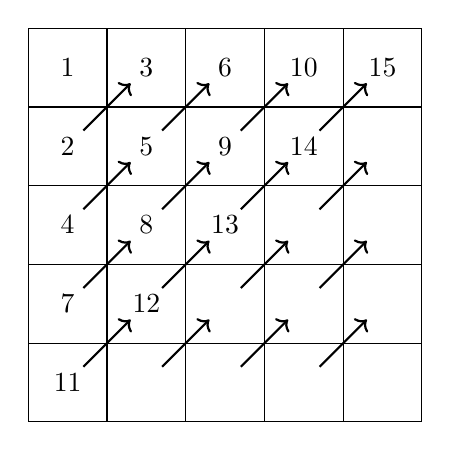
\begin{tikzpicture}[scale=1]
          % Grid
          \draw (0,0) grid (5,5);
          
          % Numbers specified (top-right triangle)
          \node at (0.5,4.5) {1};
          \node at (1.5,4.5) {3};
          \node at (2.5,4.5) {6};
          \node at (3.5,4.5) {10};
          \node at (4.5,4.5) {15};
          
          \node at (0.5,3.5) {2};
          \node at (1.5,3.5) {5};
          \node at (2.5,3.5) {9};
          \node at (3.5,3.5) {14};
          
          \node at (0.5,2.5) {4};
          \node at (1.5,2.5) {8};
          \node at (2.5,2.5) {13};
          
          \node at (0.5,1.5) {7};
          \node at (1.5,1.5) {12};
          
          \node at (0.5,0.5) {11};
          
          % Diagonal arrows
          \foreach \x in {0,...,3} {
              \foreach \y in {0,...,3} {
                  \draw[->, thick] (\x+0.7,\y+0.7) -- (\x+1.3,\y+1.3);
              }
          }
        \end{tikzpicture}
        \caption{You can see that given $(x, y)$ it is on the $(x+y+1)$th diagonal, which starts from the $\frac{1}{2} \big((x+y+1)^2 - (x+y+1) + 2)$th number and increments by $x-1$. Therefore, we have the formula above. } 
        \label{fig:rationals_countable}
      \end{figure}
    \end{proof}

  \subsection{Real Numbers} 

    The construction of the real numbers is done in my real analysis notes. We will prove the uncountability of the reals assuming you know the construction. 

    \begin{theorem}[Uncountability of Infinite Binary Numbers]
      Let $A$ be the set of all sequences whose elements are the digits $0$ and $1$. Then, $A$ is uncountable. 
    \end{theorem}

    We also know that $\mathbb{R}$ is equipotent to $A$, and so the corollary follows. 

    \begin{corollary}[Uncountability of Reals]
      $\mathbb{R}$ is uncountable. 
    \end{corollary}

  \subsection{Exercises} 

    \begin{exercise}[Math 531 Spring 2025, PS1.1]
      Find a formula for the sum of the first $n$ odd numbers and prove that it is correct.
    \end{exercise}
    \begin{solution}
      I claim that $f(n) = n^2$. I prove using induction. For $n = 1$, $f(1) = n^2 = 1^2 = 1$. Now assume $f$ holds for some $k \in \mathbb{N}$. Then, the $k$th off number is $2k-1$. Therefore 
      \begin{equation}
        f(k+1) = f(k) + (2k + 1) = k^2 + 2k + 1 = (k + 1)^2
      \end{equation}
      and the formula holds for $k=1$. By the principle of induction, $f(n) = n^2$ is true for all $n \in \mathbb{N}$. 
    \end{solution}

    \begin{exercise}[Shifrin Abstract Algebra 1.1.4.C]
      We check for $n = 1$ denoting our formula as $f$. Indeed, we have 
      \begin{equation}
        f(1) = \frac{1 \cdot 2 \cdot 3}{6} = 1 = 1^2
      \end{equation} 
      For the induction step, assume that $f(k)$ is true for some $k \in \mathbb{N}$. Then, 
      \begin{align}
        f(k+1) & = f(k) + (k+1)^2 \\
               & = \frac{k (k + 1) (2k + 1)}{6} + \frac{6 (k+1)^2}{6} \\
               & = \frac{(k+1) \{ k (2k+1) + 6(k+1)\}}{6} \\
               & = \frac{(k+1) (2k^2 + 7k + 6)}{6} \\
               & = \frac{(k+1)(k+2)(2(k+1) + 1)}{6} \\
               & = f(k+1)
      \end{align}
      Therefore $f$ holds for all $n \in \mathbb{N}$. 
    \end{exercise} 

    \begin{exercise}[Shifrin Abstract Algebra 1.1.4.G]
      We prove the base cases for $n = 1, 2, 3$. 
      \begin{enumerate}
        \item $n = 1$. $n+2 = 3$ is divisible by $3$. 
        \item $n = 2$. $n+4 = 6$ is divisible by $3$. 
        \item $n = 3$. $n+2 = 3$ is divisible by $3$. 
      \end{enumerate} 
      For our inductive step, assume that for some $n = k \in \mathbb{N}$, one of the elements in $S_k = \{k, k+2, k+4\}$ is divisible by $3$. Let us denote this element $a$. We wish to show that this claim is true for $n = k+3$ on the set $S_{k+3} = \{k+3, k+5, k+7\}$. Since $a \in S_k$, this means that $a+3 \in S_{k+3}$, and $3 | a \implies 3 | (a+3)$. So we can always identify the element $a+3$. Since we proved the base cases for $n=1, 2, 3$, and proved the recursive step, we have essentially proved the claim for all naturals of the form $3k+1, 3k+3, 3k+3$ ($k \in \mathbb{N}_0$), which is precisely the natural numbers. 
    \end{exercise}

    \begin{exercise}[Shifrin Abstract Algebra 1.1.4.J]
      Let $n = 1$. Then $1 + x \geq 1 + x$ trivially. For the induction step, assume that this inequality holds for some $n \in \mathbb{N}$. Then, we have 
      \begin{align}
        1 + (n+1) x & = 1 + nx + x \\
                    & \leq (1+x)^n + x \\ 
                    & \leq (1+x)^n + x(1+x)^n \\
                    & = (1+x)^{n+1}
      \end{align} 
      where the prove the penultimate step by applying the ordered field axioms to the 2 cases: 
      \begin{enumerate}
        \item If $x \geq 0$, then addition preserves order so $1 + x \geq 0 + 1 = 1$. Since $1 + x, 1 > 0$, order is preserved under multiplication by a positive element, so $(1+x)^2 \geq 1+x \geq 1$. Using induction, we can show that for all $n \in \mathbb{N}$, $(1+x)^n \geq 1$, and again by preservation of order under multiplication by a positive element, this implies $x (1 + x)^n \geq x$ for all $n \in \mathbb{N}$. 
        \item If $0 > x > -1$, we have $0 < 1 + x < 1$ and by the same induction proof, we can bound $0 < (1+x)^n < 1$ for all $n$. Finally by reversal of order under multiplication by a negative element, we have $x (1+x)^n > x$. 
      \end{enumerate}
      Therefore, we take the less restrictive of the 2 bounds: $x(1+x)^n \geq x$. 
    \end{exercise}

    \begin{exercise}[Shifrin Abstract Algebra 1.1.7]
      Let us denote 
      \begin{equation}
        x = \frac{1 + \sqrt{5}}{2} , \;\;\; y = \frac{1 - \sqrt{5}}{2}
      \end{equation} 
      Note the identities 
      \begin{align}
        x^2 & = \bigg( \frac{1 + \sqrt{5}}{2} \bigg)^2 = \frac{3 + 2 \sqrt{5}}{2} = 1 + x \\
        y^2 & = \bigg( \frac{1 - \sqrt{5}}{2} \bigg)^2 = \frac{3 - 2 \sqrt{5}}{2} = 1 + y
      \end{align}
      We check the base case for $n = 1$
      \begin{equation}
        a_1 = \frac{1}{\sqrt{5}} (x + y) = \frac{1}{\sqrt{5}} \frac{2 \sqrt{5}}{2} = 1
      \end{equation} 
      and for $n = 2$ 
      \begin{equation}
        a_2 = \frac{1}{\sqrt{5}} (x^2 - y^2) = \frac{1}{\sqrt{5}} ((1+x) - (1+y)) = \frac{1}{\sqrt{5}} (x + y) = a_1 = 1
      \end{equation}
      For the inductive step, assume that this formula holds for some $k-1, k \in \mathbb{N}$. Then, we have 
      \begin{align}
        a_{k+1} & = a_{k} + a_{k-1} \\
                & = \frac{1}{\sqrt{5}} (x^{k-1} - y^{k-1}) + \frac{1}{\sqrt{5}} (x^k - y^k) \\
                & = \frac{1}{\sqrt{5}} \big\{ x^{k-1} (1 + x) - y^{k-1} (1 + y)\big\} \\
                & = \frac{1}{\sqrt{5}} (x^{k+1} - y^{k+1})
      \end{align}
      and we are done. 
    \end{exercise}

\end{document}
